% questions.tex —— 2015 年·天津卷·理科 · 题目内容片段（无答案）
% 由 tools/generate_projects.py 依来源总账自 2015/2015_数学真题_天津理_试题.md 生成，勿手改（改源 MD 后重跑）


\gkpart{数学}

\begin{gktip}
\textbf{来源说明}：本题面依据固定源 PDF 全 2 页逐题核对（p1＝页 985：栏 1 标题与「一、选择题」1–5（含第 3 题框图、第 5 题圆图）；栏 2 第 5 题选项（栏首）与第 6–8 题＋「二、填空题」9–14（含第 10 题三视图）；栏 3「三、解答题」15、16；p2＝页 986：栏 1 第 17 题（含四棱柱图）、第 18 题；栏 2 第 19 题；栏 3 第 20 题）。原卷为 \textbf{A3 横向（1190.55 \(\times\) 841.89 pt）三栏书刊合排}，阅读序＝左→中→右；\textbf{页脚仅印合订本书页页码 985／986}（页面底部正中），\textbf{无页眉}。标题「2015 普通高等学校招生考试（天津卷理）」在栏 1 内排印。\textbf{全卷不印分值、不印题量、不印「考生注意」栏}——三处节头逐字仅「一、选择题」「二、填空题」「三、解答题」；总分 150 为结构推断，\textbf{卷面无凭据}，本文件不作补写。

\textbf{源制作体系判定}（\texttt{pdffonts}／\texttt{pdftotext -layout}／\texttt{pdfimages -list} 实测）：源\textbf{不是扫描件，而是 LaTeX（Computer Modern 系）重排产物}——\texttt{pdfimages -list} 零命中（全页无位图，无 Type3 字体）；嵌入字体含中文 \textbf{STSong（宋体正文）／STHeiti（黑体标题、节头与框图内汉字）}，拉丁与数学 \textbf{LMRoman 系与 CM 系（CMR10／CMMI10／CMSY10／CMEX10／MSAM10／CMR7／CMMI7／CMSY7 等）}，另有 \textbf{TeX-vect10}（专供向量长箭头绘制）。文本层整体可读；根号上划线、作答空线、\textbf{「$\parallel$」（第 14、17 题）}、全部箭头与向量箭杆均为矢量路径（「$\parallel$」实测为\textbf{两条平行矢量短斜线}：各 9.98 pt、水平偏移 2.10 pt，文本层完全丢失该符号）。

\textbf{标点与字样约定（实测）}：① \textbf{题号与句末}源内为半角 \texttt{.}（LMRoman10 出字），按全库约定写作全角「．」；② \textbf{正文句读}源内为\textbf{半角与全角混用}——第 9–15、17、18、20 题多用半角 ASCII（\texttt{,} \texttt{.} \texttt{;} \texttt{:}，LMRoman10 出字、后随字距空隙），第 10、12、13、14、16、19 题汉语小句用全角「，」（即\textbf{同一卷内两种标点并存，系源排印自身不一致}），本文件按全库约定\textbf{一律归一为全角}「，」「：」「；」「？」「（）」，内容零改动（源形在转录稿登记）；③ \textbf{引号「“”」}为全角 STSong 出字（第 4、16 题），照源保留；④ \textbf{选项标号}源内为\textbf{半角「(A)」照录}；⑤ \textbf{作答空}：填空题为统一长度横线（实测 \textbf{31.50 pt}，写作 \texttt{\gkblank{}}），选择题作答括注按全库约定写作「（　）」（源为半角括号＋ TJ 负调距 $-$999.952 撑开）；⑥ \textbf{分数}源内均为显示风格（真分式；第 12 题括号内、第 13 题 \(\cos A\) 后、第 18 题 \(b_n\) 定义式等均实测竖排两行），排印一律按显示风格（如 \(\dfrac{a}{b}\)）；⑦ \textbf{不等号}按 MSAM10 实测字形排 \(\geqslant\)／\(\leqslant\)（字形名 \texttt{greaterorequalslant}／\texttt{lessorequalslant}，U+2A7E／U+2A7D）；⑧ \textbf{向量}：本卷源\textbf{无 CMMIB10}——向量字母为 \textbf{CMMI10 常规数学斜体}、箭杆为 \textbf{TeX-vect10 长箭头}，一律录作 \(\overrightarrow{BE}\) 类（\textbf{不加粗斜体向量记号}）；⑨ \textbf{常数与函数名}：\(\log\)／\(\sin\)／\(\cos\) 源为\textbf{正体}（CMR10），照录正体；实数集与正整数集源为\textbf{粗正体}（LMRoman10-Bold），录作 \(\mathbf{R}\)／\(\mathbf{N}^{*}\)（上标星实测 U+2217）；补集号 \(\complement\) 出自 MSAM10（字形名 \texttt{complement}，U+2201）；⑩ \textbf{第 18 题}的 \(a_n\) 下标与递推式照源；⑪ \textbf{词间空格}照页面词界补。

\textbf{存疑与登记}（源内异常一律照录；完整清单见工作档 \texttt{figure-inventory.md} 存疑表 S-1…S-13 与转录稿存疑表）：① \textbf{固定源不附参考答案}（等级 D）——本题面无答案区，解析全部由本库独立推导；② \textbf{第 3 题框图为新拓扑}：初值链 \(S=20,i=1\)、步进 \(i=2i\)（翻倍型）、判据 \(i>5?\)——与常见「\(i=i+1\)」变体不同，逐字照源复刻（「否」支自菱形右顶点三段回折汇入主干）；③ \textbf{第 5 题的四个选项排在本卷栏 2 之首}（位于第 6 题题文之上）——系三栏合排的断栏排版：题干与圆图在栏 1 末、选项续排于栏 2 首；归属裁定依据为内容流绘制次序（题干→圆图→选项→Q6 题文）与数学一致性（按相交弦定理独立求解可验证归并无误），\textbf{本文件按题归并}；④ \textbf{第 14、17 题的「$\parallel$」}为矢量短斜线、文本层丢失——按语义排印 \(\parallel\)；⑤ \textbf{第 6 题抛物线}实测为 \(y^2=4\sqrt{7}x\)（400\% 放大核对照源）；⑥ \textbf{第 8 题分段函数内两种不等号形态并存}（\(x\leqslant2\) 为 MSAM10 斜杠型、\(x>2\) 为 CMMI10 直立型，属源字形，照源）；⑦ \textbf{第 2 题题文折行}系约束条件组下延所致，本文件按语序归并；⑧ 全卷无分值印制，不录不补。
\end{gktip}

\gkpart{试题}

\gkpart{一、选择题}

\begin{question}
\gkti{1}已知全集 \(U=\{1,2,3,4,5,6,7,8\}\)，集合 \(A=\{2,3,5,6\}\)，集合 \(B=\{1,3,4,6,7\}\)，则集合 \(A\cap\complement_U B=\)（　）

(A) \(\{2,5\}\)　(B) \(\{3,6\}\)　(C) \(\{2,5,6\}\)　(D) \(\{2,3,5,6,8\}\)

\end{question}
\begin{question}
\gkti{2}设变量 \(x\)，\(y\) 满足约束条件 \(\begin{cases}x+2\geqslant0,\\x-y+3\geqslant0,\\2x+y-3\leqslant0,\end{cases}\) 则目标函数 \(z=x+6y\) 的最大值为（　）

(A) 3　(B) 4　(C) 18　(D) 40

\Needspace{0.4\textheight}
\end{question}
\begin{question}
\gkti{3}阅读程序框图，运行相应的程序，则输出 \(S\) 的值为（　）
\nopagebreak[4]
\begin{center}% ============================================================
% f2015tjl_q03_flowchart.tex —— 2015 天津卷（理科）第 3 题 程序框图
% ------------------------------------------------------------
% 坐标口径：图内画布 pt，原点 = 源页基准点，x 右正、y 上正。
%   来源：.work/phase3-b11/figure-inventory.md（真实页 pt，原点左上、y 向下）
%   换算：X_tikz = x_page − 179.30 ；  Y_tikz = 533.77 − y_page
% 线宽：图形本体 0.398 pt（清单 §1.2）。
% 箭头：TikZ arrows.meta 标准箭矢（> = Triangle），箭尖落于清单所给尖端坐标；
%       源图线段本体短于尖端（留白由填充三角补齐），TikZ 由 tip 自动收尾，等效。
% 标签：绝对字号 10.5pt / 行距 12.6pt，inner sep=0（全库既定，勿改相对字号）。
% 要素：7 框 + 6 主干 + 1 回折 = 14 描边 path；7 填充箭头（清单 §1.5 合计 21）。
% ============================================================
\usetikzlibrary{arrows.meta}
\begin{tikzpicture}[
  x=1pt,y=1pt,                             % 画布单位 = 1 pt（本文件坐标一律为 pt）
  every node/.style={font=\fontsize{10.5pt}{12.6pt}\selectfont,inner sep=0pt},
  >={Triangle[length=3.60pt,width=3.36pt]},
  fr/.style={line width=0.398pt},          % 框体
  ln/.style={line width=0.398pt},          % 主干 / 回折线
]

  % ---------- 主干线（x = 216.22 → 36.92；起笔点在段首，箭尖在段尾）----------
  \draw[ln,->] (36.92,184.78) -- (36.92,170.61);   % a 开始 → S=20,i=1
  \draw[ln,->] (36.92,154.01) -- (36.92,139.84);   % b S=20,i=1 → i=2i
  \draw[ln,->] (36.92,125.52) -- (36.92,111.34);   % c i=2i → S=S−i
  \draw[ln,->] (36.92, 95.89) -- (36.92, 81.72);   % d S=S−i → 菱形
  \draw[ln,->] (36.92, 62.82) -- (36.92, 48.64);   % e 菱形下顶点 → 输出 S
  \draw[ln,->] (36.92, 31.38) -- (36.92, 17.21);   % f 输出 S → 结束

  % ---------- 「否」支回折（3 段：右 → 上 → 左），自菱形右顶点右侧 0.28 起笔 ----------
  \draw[ln,->] (74.13,72.27) -- (88.31,72.27) -- (88.31,146.93) -- (36.92,146.93);

  % ---------- 节点框 ----------
  % 1 开始（圆角矩形，r≈3.99）
  \draw[fr,rounded corners=3.99pt] (22.92,184.98) rectangle (50.92,201.82);
  \node at (36.90,193.97) {开始};
  % 2 S=20, i=1
  \draw[fr] (3.01,154.21) rectangle (70.84,170.41);
  \node at (36.925,162.31) {$S=20,\,i=1$};
  % 3 i=2i
  \draw[fr] (20.18,125.72) rectangle (53.67,139.64);
  \node at (36.925,132.68) {$i=2i$};
  % 4 S=S−i
  \draw[fr] (11.15,96.09) rectangle (62.69,111.14);
  \node at (36.92,103.615) {$S=S-i$};
  % 5 i>5?（菱形，右/上/左/下顶点）
  \draw[fr] (73.85,72.27) -- (36.92,81.44) -- (0.00,72.27) -- (36.92,63.10) -- cycle;
  \node at (36.92,72.27) {$i>5?$};
  % 6 输出 S（非直角平行四边形，顶部右斜 6.14）
  \draw[fr] (11.51,31.58) -- (17.65,48.44) -- (62.33,48.44) -- (56.19,31.58) -- cycle;
  \node at (36.92,40.01) {输出 $S$};
  % 7 结束（圆角矩形，r≈3.99）
  \draw[fr,rounded corners=3.99pt] (22.92,0.00) rectangle (50.92,17.01);
  \node at (36.90,9.07) {结束};

  % ---------- 支标（清单 §1.4 实测字形中心）----------
  \node at (45.90,56.37) {是};
  \node at (74.10,64.57) {否};

\end{tikzpicture}
\end{center}
\nopagebreak[4]
(A) \(-10\)　(B) 6　(C) 14　(D) 18

\end{question}
\begin{question}
\gkti{4}设 \(x\in\mathbf{R}\)，则“\(|x-2|<1\)”是“\(x^2+x-2>0\)”的（　）

(A) 充分而不必要条件　(B) 必要而不充分条件

(C) 充要条件　(D) 既不充分也不必要条件

\Needspace{0.4\textheight}
\end{question}
\begin{question}
\gkti{5}如图，在圆 \(O\) 中，\(M\)，\(N\) 是弦 \(AB\) 的三等分点，弦 \(CD\)，\(CE\) 分别经过点 \(M\)，\(N\)，若 \(CM=2\)，\(MD=4\)，\(CN=3\)，则线段 \(NE\) 的长为（　）
\nopagebreak[4]
\begin{center}% ============================================================
% f2015tjl_q05_circle.tex —— 2015 天津卷（理科）第 5 题 圆与割线
% ------------------------------------------------------------
% 坐标口径：图内画布 pt，原点 = 源页基准点，x 右正、y 上正。
%   来源：.work/phase3-b11/figure-inventory.md（真实页 pt，原点左上、y 向下）
%   换算：X_tikz = x_page − 169.40 ；  Y_tikz = 773.78 − y_page
% 线宽：圆 0.398 pt；弦 AB 0.398 pt（图形本体档，清单未单独标注，取本体档）；
%       两割线 CE / CD **0.42 pt**（清单 §2.3 实测值，源图自身与他线不同档，照源保留）。
% 照源复刻（清单 §7 存疑）：
%   S-3 圆心实心点为**字形** U+2022（\textbullet），非矢量填充；与「O」并置为「•O」，
%       字形落于文字基线，其墨迹中心较几何圆心 (53.895,53.890) 有约 3.6 pt 垂直偏置。
%   S-4 两割线在弦高 y=736.90 处与三等分点 M/N 有 1.65 / 0.49 pt 微差（源图未精确
%       满足题设交点约束）——**照源复刻，不「修正」**。
% 要素：3 描边 path（圆 / 弦 / 两割线合一）+ 8 文字标签（清单 §2.6）。
% ============================================================
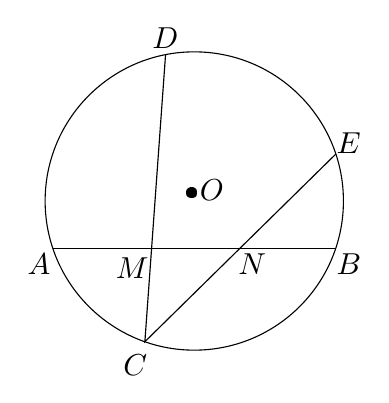
\begin{tikzpicture}[
  x=1pt,y=1pt,                             % 画布单位 = 1 pt（本文件坐标一律为 pt）
  every node/.style={font=\fontsize{10.5pt}{12.6pt}\selectfont,inner sep=0pt},
  body/.style={line width=0.398pt},
  sec/.style={line width=0.420pt},
]

  % ---------- 圆（圆心 (223.295,719.890)，r = 53.895）----------
  \draw[body] (53.895,53.890) circle [radius=53.895pt];

  % ---------- 弦 AB（水平全长弦，(172.10,736.90)→(274.50,736.90)，长 102.40）----------
  \draw[body] (2.70,36.88) -- (105.10,36.88);

  % ---------- 两割线（源图为 1 个 path 的 2 个子段，共点 C）----------
  % CE：E(274.49,702.88) → C(205.44,770.75)
  % CD：C(205.44,770.75) → D(212.92,666.99)
  \draw[sec] (105.09,70.90) -- (36.04,3.03) -- (43.52,106.79);

  % ---------- 标签（清单 §2.5 实测字形中心）----------
  \node at (-2.20,30.98)  {$A$};
  \node at (109.80,30.98) {$B$};
  \node at (32.60,-5.32)  {$C$};
  \node at (43.40,112.78) {$D$};
  \node at (109.70,74.88) {$E$};
  \node at (31.50,29.58)  {$M$};
  \node at (74.80,30.98)  {$N$};

  % ---------- 圆心「•O」：U+2022 字形与 O 并置（S-3 照源）----------
  \node at (57.495,57.86) {\textbullet $O$};

\end{tikzpicture}
\end{center}
\nopagebreak[4]
(A) \(\dfrac{8}{3}\)　(B) 3　(C) \(\dfrac{10}{3}\)　(D) \(\dfrac{5}{2}\)

\end{question}
\begin{question}
\gkti{6}已知双曲线 \(\dfrac{x^2}{a^2}-\dfrac{y^2}{b^2}=1\)（\(a>0\)，\(b>0\)）的一条渐近线过点 \((2,\sqrt{3})\)，且双曲线的一个焦点在抛物线 \(y^2=4\sqrt{7}x\) 的准线上，则双曲线的方程为（　）

(A) \(\dfrac{x^2}{21}-\dfrac{y^2}{28}=1\)　(B) \(\dfrac{x^2}{28}-\dfrac{y^2}{21}=1\)

(C) \(\dfrac{x^2}{3}-\dfrac{y^2}{4}=1\)　(D) \(\dfrac{x^2}{4}-\dfrac{y^2}{3}=1\)

\end{question}
\begin{question}
\gkti{7}已知定义在 \(\mathbf{R}\) 上的函数 \(f(x)=2^{|x-m|}-1\)（\(m\) 为实数）为偶函数，记 \(a=f(\log_{0.5}3)\)，\(b=f(\log_2 5)\)，\(c=f(2m)\)，则 \(a\)，\(b\)，\(c\) 的大小关系为（　）

(A) \(a<b<c\)　(B) \(a<c<b\)　(C) \(c<a<b\)　(D) \(c<b<a\)

\end{question}
\begin{question}
\gkti{8}已知函数 $f(x)=\begin{cases}2-|x|,&x\leqslant2,\\(x-2)^2,&x>2,\end{cases}$ 函数 \(g(x)=b-f(2-x)\)，其中 \(b\in\mathbf{R}\)．若函数 \(y=f(x)-g(x)\) 恰有 4 个零点，则 \(b\) 的取值范围是（　）

(A) \(\left(\dfrac{7}{4},+\infty\right)\)　(B) \(\left(-\infty,\dfrac{7}{4}\right)\)　(C) \(\left(0,\dfrac{7}{4}\right)\)　(D) \(\left(\dfrac{7}{4},2\right)\)

\end{question}
\gkpart{二、填空题}

\begin{question}
\gkti{9}\(\mathrm{i}\) 是虚数单位，若复数 \((1-2\mathrm{i})(a+\mathrm{i})\) 是纯虚数，则实数 \(a\) 的值为\gkblank{}．

\Needspace{0.4\textheight}
\end{question}
\begin{question}
\gkti{10}一个几何体的三视图如图所示（单位：m），则该几何体的体积为\gkblank{}m³．
\nopagebreak[4]
\begin{center}% ============================================================
% f2015tjl_q10_views.tex —— 2015 天津卷（理科）第 10 题 三视图
% ------------------------------------------------------------
% 坐标口径：图内画布 pt，原点 = 源页基准点，x 右正、y 上正。
%   来源：.work/phase3-b11/figure-inventory.md（真实页 pt，原点左上、y 向下）
%   换算：X_tikz = x_page − 493.36 ；  Y_tikz = 573.70 − y_page
% 比例基准：源题「1」= 28.35 pt（清单 §3），全图尺寸标注均为其整数倍。
% 线宽：图形本体 0.398 pt（轮廓 / 分隔线 / 尺寸线 / 界限短线统一本档）。
% 箭头：TikZ arrows.meta 标准箭矢（> = Triangle）；尺寸线每段一枚实心三角，
%       箭尖落在段尾坐标（= 清单所列「起点→终点」的终点，指向最近的尺寸界限线）。
% 照源复刻（清单 §7 存疑）：
%   S-5 俯视图**无水平尺寸线**（正视图有「1 | 2 | 1」三条）——不补。
%   S-6 侧视图半径线本体止于 (196.09,159.24)，箭尖 (198.63,161.78) 至圆心 28.35 = 恰好 1 图；
%       「线段长」与「半径」口径不一致——照源，半径以尖端计。
% 要素：46 描边 path（正视 27 + 侧视 2 + 俯视 17）+ 23 填充箭头（14 + 1 + 8）
%       + 9 文字标签（清单 §3.5 B 表、§3.4）。
% ============================================================
\usetikzlibrary{arrows.meta}
\begin{tikzpicture}[
  x=1pt,y=1pt,                             % 画布单位 = 1 pt（本文件坐标一律为 pt）
  every node/.style={font=\fontsize{10.5pt}{12.6pt}\selectfont,inner sep=0pt},
  >={Triangle[length=3.60pt,width=3.36pt]},
  g/.style={line width=0.398pt},
]

  % =========================================================
  % 正视图（上左）
  % =========================================================
  % 轮廓（6 点六边形：中央 2 图×2 图矩形 + 左右各伸 1 图三角尖）
  \draw[g] (8.50,141.74) -- (36.85,113.39) -- (93.54,113.39) -- (121.89,141.74)
           -- (93.54,170.08) -- (36.85,170.08) -- cycle;
  % 内部分隔竖线
  \draw[g] (36.85,113.39) -- (36.85,170.08);
  \draw[g] (93.54,113.39) -- (93.54,170.08);
  % 尺寸箭头：竖直 · 右外 @ X=127.56（每组「1」上下各一枚，箭尖朝外）
  \draw[g,->] (127.56,121.89) -- (127.56,116.98);
  \draw[g,->] (127.56,133.23) -- (127.56,138.15);
  \draw[g,->] (127.56,150.24) -- (127.56,145.32);
  \draw[g,->] (127.56,161.58) -- (127.56,166.50);
  % 尺寸箭头：竖直 · 左外 @ X=2.83
  \draw[g,->] (2.83,121.89) -- (2.83,116.98);
  \draw[g,->] (2.83,133.23) -- (2.83,138.15);
  \draw[g,->] (2.83,150.24) -- (2.83,145.32);
  \draw[g,->] (2.83,161.58) -- (2.83,166.50);
  % 尺寸箭头：水平 · 下方 @ Y=107.72（三段读数 1 | 2 | 1）
  \draw[g,->] (17.00,107.72) -- (12.09,107.72);
  \draw[g,->] (28.34,107.72) -- (33.26,107.72);
  \draw[g,->] (59.52,107.72) -- (40.43,107.72);
  \draw[g,->] (70.86,107.72) -- (89.95,107.72);
  \draw[g,->] (102.04,107.72) -- (97.13,107.72);
  \draw[g,->] (113.38,107.72) -- (118.30,107.72);
  % 尺寸界限短线：左外 3 条 / 右外 3 条
  \draw[g] (5.67,113.39) -- (0.00,113.39);
  \draw[g] (5.67,141.74) -- (0.00,141.74);
  \draw[g] (5.67,170.08) -- (0.00,170.08);
  \draw[g] (124.72,113.39) -- (130.39,113.39);
  \draw[g] (124.72,141.74) -- (130.39,141.74);
  \draw[g] (124.72,170.08) -- (130.39,170.08);
  % 尺寸界限短线：下方竖短线 4 条 @ 轮廓四角 x
  \draw[g] (8.50,110.55)  -- (8.50,104.89);
  \draw[g] (36.85,110.55) -- (36.85,104.89);
  \draw[g] (93.54,110.55) -- (93.54,104.89);
  \draw[g] (121.89,110.55) -- (121.89,104.89);
  % 读数与图名
  \node at (22.64,107.00)  {1};
  \node at (65.24,107.00)  {2};
  \node at (107.74,107.00) {1};
  \node at (2.84,155.20)   {1};
  \node at (2.84,126.80)   {1};
  \node at (127.54,155.20) {1};
  \node at (127.54,126.80) {1};
  \node at (65.24,91.30)   {正视图};

  % =========================================================
  % 侧视图（上右）：半径 1 图圆 + 半径引导线
  % =========================================================
  \draw[g] (178.58,141.74) circle [radius=28.35pt];
  \draw[g,->] (178.58,141.74) -- (198.63,161.78);
  \node at (192.74,143.80) {1};
  \node at (178.54,91.30)  {侧视图};

  % =========================================================
  % 俯视图（下左）：与正视图同形同尺寸，沿 y 下移 113.39
  % =========================================================
  \draw[g] (8.50,28.35) -- (36.85,0.00) -- (93.54,0.00) -- (121.89,28.35)
           -- (93.54,56.70) -- (36.85,56.70) -- cycle;
  \draw[g] (36.85,0.00) -- (36.85,56.70);
  \draw[g] (93.54,0.00) -- (93.54,56.70);
  % 尺寸箭头：竖直 · 右外 @ X=127.56
  \draw[g,->] (127.56,8.51)  -- (127.56,3.59);
  \draw[g,->] (127.56,19.84) -- (127.56,24.76);
  \draw[g,->] (127.56,36.85) -- (127.56,31.93);
  \draw[g,->] (127.56,48.19) -- (127.56,53.11);
  % 尺寸箭头：竖直 · 左外 @ X=2.83
  \draw[g,->] (2.83,8.51)  -- (2.83,3.59);
  \draw[g,->] (2.83,19.84) -- (2.83,24.76);
  \draw[g,->] (2.83,36.85) -- (2.83,31.93);
  \draw[g,->] (2.83,48.19) -- (2.83,53.11);
  % 尺寸界限短线：左外 3 条 / 右外 3 条（照源无水平尺寸线，S-5）
  \draw[g] (5.67,0.00)  -- (0.00,0.00);
  \draw[g] (5.67,28.35) -- (0.00,28.35);
  \draw[g] (5.67,56.70) -- (0.00,56.70);
  \draw[g] (124.72,0.00)  -- (130.39,0.00);
  \draw[g] (124.72,28.35) -- (130.39,28.35);
  \draw[g] (124.72,56.70) -- (130.39,56.70);
  % 读数与图名
  \node at (2.84,41.80)   {1};
  \node at (2.84,13.40)   {1};
  \node at (127.54,41.80) {1};
  \node at (127.54,13.40) {1};
  \node at (65.24,-13.50) {俯视图};

\end{tikzpicture}
\end{center}
\nopagebreak[4]
\end{question}
\begin{question}
\gkti{11}曲线 \(y=x^2\) 与直线 \(y=x\) 所围成的封闭图形的面积为\gkblank{}．

\end{question}
\begin{question}
\gkti{12}在 \(\left(x-\dfrac{1}{4x}\right)^6\) 的展开式中，\(x^2\) 的系数为\gkblank{}．

\end{question}
\begin{question}
\gkti{13}在 \(\triangle ABC\) 中，内角 \(A\)，\(B\)，\(C\) 所对的边分别为 \(a\)，\(b\)，\(c\)．已知 \(\triangle ABC\) 的面积为 \(3\sqrt{15}\)，\(b-c=2\)，\(\cos A=-\dfrac{1}{4}\)，则 \(a\) 的值为\gkblank{}．

\end{question}
\begin{question}
\gkti{14}在等腰梯形 \(ABCD\) 中，已知 \(AB\parallel DC\)，\(AB=2\)，\(BC=1\)，\(\angle ABC=60^{\circ}\)．动点 \(E\) 和 \(F\) 分别在线段 \(BC\) 和 \(DC\) 上，且 \(\overrightarrow{BE}=\lambda\overrightarrow{BC}\)，\(\overrightarrow{DF}=\dfrac{1}{9\lambda}\overrightarrow{DC}\)，则 \(\overrightarrow{AE}\cdot\overrightarrow{AF}\) 的最小值为\gkblank{}．

\end{question}
\gkpart{三、解答题}

\begin{question}
\gkti{15}已知函数 \(f(x)=\sin^2 x-\sin^2\left(x-\dfrac{\pi}{6}\right)\)，\(x\in\mathbf{R}\)．

（1） 求 \(f(x)\) 的最小正周期；

（2） 求 \(f(x)\) 在区间 \(\left[-\dfrac{\pi}{3},\dfrac{\pi}{4}\right]\) 上的最大值和最小值．

\end{question}
\begin{question}
\gkti{16}为推动乒乓球运动的发展，某乒乓球比赛允许不同协会的运动员组队参加．现有来自甲协会的运动员 3 名，其中种子选手 2 名；乙协会的运动员 5 名，其中种子选手 3 名．从这 8 名运动员中随机选择 4 人参加比赛．

（1） 设 \(A\) 为事件“选出的 4 人中恰有 2 名种子选手，且这 2 名种子选手来自同一个协会”，求事件 \(A\) 发生的概率；

（2） 设 \(X\) 为选出的 4 人中种子选手的人数，求随机变量 \(X\) 的分布列和数学期望．

\Needspace{0.4\textheight}
\end{question}
\begin{question}
\gkti{17}如图，在四棱柱 \(ABCD\text{-}A_1B_1C_1D_1\) 中，侧棱 \(A_1A\perp\) 底面 \(ABCD\)，\(AB\perp AC\)，\(AB=1\)，\(AC=AA_1=2\)，\(AD=CD=\sqrt{5}\)，且点 \(M\) 和 \(N\) 分别为 \(B_1C\) 和 \(D_1D\) 的中点．
\nopagebreak[4]
\begin{center}% ============================================================
% f2015tjl_q17_prism.tex —— 2015 天津卷（理科）第 17 题 四棱柱
% ------------------------------------------------------------
% 坐标口径：图内画布 pt，原点 = 源页基准点，x 右正、y 上正。
%   来源：.work/phase3-b11/figure-inventory.md（真实页 pt，原点左上、y 向下）
%   换算：X_tikz = x_page − 236.74 ；  Y_tikz = 329.48 − y_page
% 线宽：全图 0.3985 pt；**虚线节距 2.98883 / 2.98883**（全卷唯一虚线组，清单 §0.4）。
% 实/虚分工：实线 11 条、虚线 7 条（清单 §4.2）。底面四边形 D-C-B-A，A 为被遮挡顶点，
%   故 BC、CD 实线，DA、AB 与对角线 AC 均虚线；一切以 A 为端点的线（AA₁/AB/AC/AD/AB₁/AD₁）
%   皆虚线，与「A 在后」一致。
% N = D₁D 中点 (0.00,81.36)；M = B₁C 中点 (101.01,63.70)，N–M 连线为虚线。
% 照源复刻（清单 §7）：S-7 题设「设 E 为棱 A₁B₁ 上的点」，而**源图未画出 E 点**——不补。
% 要素：18 描边 path（实 11 + 虚 7），填充路径 0；顶点标签 8 + 中点标签 2（清单 §4.4）。
% ============================================================
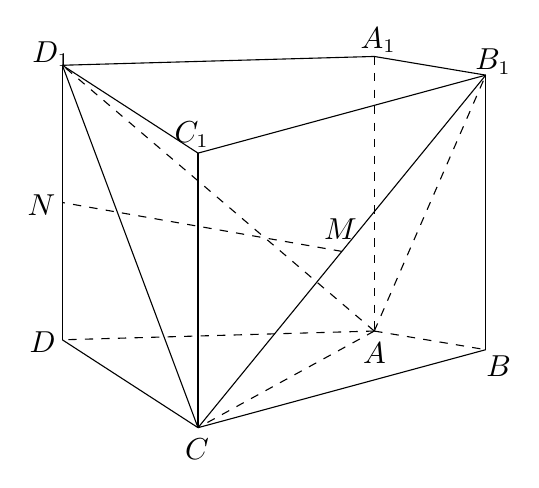
\begin{tikzpicture}[
  x=1pt,y=1pt,                             % 画布单位 = 1 pt（本文件坐标一律为 pt）
  every node/.style={font=\fontsize{10.5pt}{12.6pt}\selectfont,inner sep=0pt},
  s/.style={line width=0.3985pt},
  d/.style={line width=0.3985pt,dash pattern=on 2.98883pt off 2.98883pt},
]

  % ---------- 实线 11 条 ----------
  \draw[s] (0.00,130.96) -- (0.00,31.75);       % 1  D₁D
  \draw[s] (49.02,99.21) -- (49.02,0.00);       % 2  C₁C
  \draw[s] (112.71,134.14) -- (152.99,127.39);  % 3  A₁B₁
  \draw[s] (152.99,127.39) -- (49.02,99.21);    % 4  B₁C₁
  \draw[s] (49.02,99.21) -- (0.00,130.96);      % 5  C₁D₁
  \draw[s] (0.00,130.96) -- (112.71,134.14);    % 6  D₁A₁
  \draw[s] (49.02,0.00) -- (0.00,130.96);       % 7  D₁C
  \draw[s] (49.02,0.00) -- (152.99,127.39);     % 8  B₁C
  \draw[s] (152.99,127.39) -- (152.99,28.18);   % 9  B₁B
  \draw[s] (0.00,31.75) -- (49.02,0.00);        % 10 DC
  \draw[s] (49.02,0.00) -- (152.99,28.18);      % 11 CB

  % ---------- 虚线 7 条 ----------
  \draw[d] (112.71,134.14) -- (112.71,34.92);   % 12 A₁A
  \draw[d] (112.71,34.92) -- (152.99,28.18);    % 13 AB
  \draw[d] (112.71,34.92) -- (49.02,0.00);      % 14 AC
  \draw[d] (112.71,34.92) -- (0.00,31.75);      % 15 AD
  \draw[d] (112.71,34.92) -- (152.99,127.39);   % 16 AB₁
  \draw[d] (112.71,34.92) -- (0.00,130.96);     % 17 AD₁
  \draw[d] (101.01,63.70) -- (0.00,81.36);      % 18 NM（M → N）

  % ---------- 标签（清单 §4.1 / §4.3 实测字形中心）----------
  \node at (-4.04,134.98)  {$D_1$};
  \node at (114.16,139.98) {$A_1$};
  \node at (155.66,132.18) {$B_1$};
  \node at (46.76,105.98)  {$C_1$};
  \node at (-7.14,30.78)   {$D$};
  \node at (112.76,26.98)  {$A$};
  \node at (157.66,22.28)  {$B$};
  \node at (48.66,-7.92)   {$C$};
  \node at (-7.54,80.38)   {$N$};
  \node at (100.46,71.68)  {$M$};

\end{tikzpicture}
\end{center}
\nopagebreak[4]
（1） 求证：\(MN\parallel\) 平面 \(ABCD\)；

（2） 求二面角 \(D_1\text{-}AC\text{-}B_1\) 的正弦值；

（3） 设 \(E\) 为棱 \(A_1B_1\) 上的点，若直线 \(NE\) 和平面 \(ABCD\) 所成角的正弦值为 \(\dfrac{1}{3}\)，求线段 \(A_1E\) 的长．

\end{question}
\begin{question}
\gkti{18}已知数列 \(\{a_n\}\) 满足 \(a_{n+2}=qa_n\)（\(q\) 为实数，且 \(q\neq1\)），\(n\in\mathbf{N}^{*}\)，\(a_1=1\)，\(a_2=2\)，且 \(a_2+a_3\)，\(a_3+a_4\)，\(a_4+a_5\) 成等差数列．

（1） 求 \(q\) 的值和 \(\{a_n\}\) 的通项公式；

（2） 设 \(b_n=\dfrac{\log_2 a_{2n}}{a_{2n-1}}\)，\(n\in\mathbf{N}^{*}\)，求数列 \(\{b_n\}\) 的前 \(n\) 项和．

\end{question}
\begin{question}
\gkti{19}已知椭圆 \(\dfrac{x^2}{a^2}+\dfrac{y^2}{b^2}=1\)（\(a>b>0\)）的左焦点为 \(F(-c,0)\)，离心率为 \(\dfrac{\sqrt{3}}{3}\)，点 \(M\) 在椭圆上且位于第一象限，直线 \(FM\) 被圆 \(x^2+y^2=\dfrac{b^2}{4}\) 截得的线段的长为 \(c\)，\(|FM|=\dfrac{4\sqrt{3}}{3}\)．

（1） 求直线 \(FM\) 的斜率；

（2） 求椭圆的方程；

（3） 设动点 \(P\) 在椭圆上，若直线 \(FP\) 的斜率大于 \(\sqrt{2}\)，求直线 \(OP\)（\(O\) 为原点）的斜率的取值范围．

\end{question}
\begin{question}
\gkti{20}已知函数 \(f(x)=nx-x^n\)，\(x\in\mathbf{R}\)，其中 \(n\in\mathbf{N}^{*}\)，且 \(n\geqslant2\)．

（1） 讨论 \(f(x)\) 的单调性；

（2） 设曲线 \(y=f(x)\) 与 \(x\) 轴正半轴的交点为 \(P\)，曲线在点 \(P\) 处的切线方程为 \(y=g(x)\)，求证：对于任意的正实数 \(x\)，都有 \(f(x)\leqslant g(x)\)；

（3） 若关于 \(x\) 的方程 \(f(x)=a\)（\(a\) 为实数）有两个正实数根 \(x_1\)，\(x_2\)，求证：\(|x_2-x_1|<\dfrac{a}{1-n}+2\)．

\end{question}